\documentclass{article}
\usepackage{graphicx}
%\usepackage{subfig}
\usepackage{amsmath}
\usepackage{mathtools}
\usepackage{cleveref}
%\usepackage{subfig}	
\usepackage{subcaption}
\usepackage[numbered,framed]{mcode}
\usepackage{fixltx2e}				% For the \textsubscript{} usage
\usepackage{textgreek}	

\author{Grupp B}
\title{FRT090 \\Feedback Seminar 1(Modeling/Design)  }				% \\ <=> NEW LINE IN LaTex
\date{November 2014}


\begin{document}
\maketitle	% prints the preamble onto the pdf
\newpage


\section {Overview over the project and its objectives}

Our system is a unicycle which will maintain the balance in two directions. The first being the pitch and the second being roll. It should maintain balance in realtime and withstand small disturbances meaning a small push in the pitch or roll direction. The system is being divided into two parts, the first being the part which will maintain the balance in the roll direction and the second which will maintain balance in the pitch direction. The realization will be a inverted pendulum with a inertia wheel at the top. While the balancing part in the pitch direction will be achieved which a wheel attached at the end of the inverted pendulum. In other words there will be two processes which will be regulated, the inverted pendulum  with the inertia wheel and the inverted pendulum with a wheel at the bottom. 



\section{Discussion on the modeling needs in the project}

\subsection{Why is modeling needed and what should models be used for}

We intend to model two processes parallel and at the end to set them together and tune them so they work together. as well. The first process we model is the inertia wheel with the rod, looks like the inverted pendulum however the bottom is stationary while the inertia wheel is at the top and can spin freely to maintain the balance for the rod to stand up straight.

The second main process is the rod with the wheel at the bottom which spin freely, as the first one this one also looks like the inverted pendulum but in this case the wheel at the bottom has the mission to maintain the balance to the rod. 

We will use our models to investigate the stability of the processes, which regulator is best suited and simulate it in Matlab with the program Simulink. Further we also intend to use our models to understand how the process acts for different parameters e.g. how stabile is our process if we move the center of gravity lower down or higher up.

More specific to the process with the inertia wheel we also need to come up with a model for the inertia wheel, the dimensions of it with other words which demention suits us best to achieve the result we desire. In this case we would want to have as much torque as possible at the same time as we want to have so low mass as possible. So in other words we want the perfect trade of of the two properties. 


\subsection{How is a model quality assessed}

The best way to find out the quality of the model is to simulate it and se if the result is reasonable with the expected result (in the easier cases if the process is to complex it is hard to predict the result). Make use of prior knowledge of similar processes.    


\section{Description of the models developed so far in the project }

% Equation describing 
\begin{equation}
		\begin{aligned}
	     	 (J_{w}+ML^2 + J_{p} ) \frac{\partial^2 \theta_{1} }{\partial t^2}  &= l_{1} \sin{\theta_{1}} m g + L \sin{\theta_{1}} M g - \tau    \\  
		 J_{w} \frac{\partial^2 \theta_{2}} {\partial t^2} &= \tau
		\end{aligned}
	 	\label{equ:inverted_pendulum}  
\end{equation}


The model we have so far is given in by equation \ref{equ:inverted_pendulum} which describes the inverted pendulum with the inertia wheel at the top. As one also can see in figure \ref{fig:sketch_inverted_pendulum} which is a sketch of the model so far. The rod is stationary while the inertia wheel can can spin around the axis of the rod at the top. So basically this is the process.

\begin{figure}
	\centering
	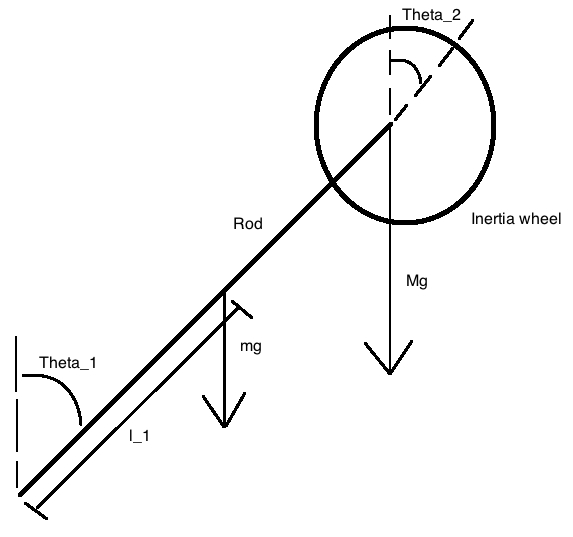
\includegraphics[width=0.7\textwidth]{Inverted_pedulum_2}
	\caption{Shows the sketch of the inverted pendulum and the meaning of the parameters.}
	\label{fig:sketch_inverted_pendulum}
\end{figure}



\section{Motivation for the selected modeling \& design approaches}

We choose to go with the Newton model which seems to be the most familiar model for us in the group due to prior knowledge with Newtons laws of forces and torques. There is other approaches which can be Lagrange's mechanics which is a essentially a statement derived from Newtons laws which simplify the work of describing more complex systems. Regarding the design approaches one would like to have some characteristics as fast response time, minimal overshoot and be able to handle disturbances for the process which can be achieved with a PID regulator. Luckily there is a way of specifying the demands and Simulink does the calculations of the parameters in the PID regulator. 


\section{Discussion on experience with respect to modeling and design}



The biggest experience was that one need to have a good model for the system to be able to find out how the process behaves and then simulate it in Simulink with Matlab to actually se where the pools are placed. But before simulating it one need to do some calculations by hand so one can compare the handwritten solution with the simulation. Because maybe in the process of simulating the process one can do mistakes, these mistakes are easy to find if one have a handwritten result to compare with.  

An another big experiencer was to build up a process description from scratch so to speak. Also called system identification which means that we found a model then the corresponding differential equation from there to the state equations. Furthermore the transfer function for the process, investigate the poles and lastly investigate the stability from the placing of the poles. So in essence the steps was not that unique but all the steps together gave us an insight how a project is built up from scratch which we find to be a unique experience. 

A last point to be made is that simulations in simulink gave us a huge advantage due to the simplicity to se all the properties of the closed loop with a PID regulator, e.g. the step response, bode plot, Nyquist digram and so in. 

\end{document}